\documentclass{article}
\usepackage[utf8]{inputenc}


\usepackage[english]{babel}
\usepackage{natbib}
\usepackage{amssymb}
\usepackage{multicol}
\usepackage[fleqn]{amsmath}
\usepackage{epsfig}
\usepackage[normalem]{ulem}
\usepackage{verbatim}
\usepackage{graphicx}
\usepackage{url} % pour ins\'erer des url
\usepackage{color}
\usepackage{dsfont}
\usepackage{amsmath,amsfonts,times,latexsym,comment,times}
\usepackage{color,epsfig,rotating}
\newcommand{\ds}{\displaystyle}
\newcommand{\bce}{\begin{center}}
\newcommand{\ece}{\end{center}}
%\usepackage{mprocl}


\def\GEV{{\cal{GEV}}} % raccourci pour la d\'enomination de la loi GEV
\def\GPD{{\cal{GPD}}} % raccourci pour la d\'enomination de la loi GPD
\def\EXPO{{\cal{E}}} % raccourci pour la d\'enomination de la loi exponentielle
\def\GAUSS{{\cal{N}}} % raccourci pour la d\'enomination de la loi gaussienne
\def\GEV{{\cal{GEV}}} % raccourci pour la d\'enomination de la loi GEV
\def\BERN{{\cal{B}}_e} % raccourci pour la d\'enomination de la loi de Bernoulli
\def\BINOM{{\cal{B}}} % raccourci pour la d\'enomination de la loi binomiale
\def\POIS{{\cal{P}}} % raccourci pour la d\'enomination de la loi de Poisson


\def\iid{\textit{iid} } % raccourci pour le terme "i.i.d."
\def\va{\textit{va} } % raccourci pour le terme "variable al\'eatoire"
\def\EMV{$\text{EMV}$} % raccourci pour le terme "estimateur du maximum de vraisemblance"
\def\EMC{$\text{EMC}$} % raccourci pour le terme "estimateur des moindres carr\'es"
\def\MSY{\mbox{MSY}} 
\def\msy{\mbox{\small{MSY}}}



\newcounter{cptpropo}[part]
\newenvironment{propo}[0]
{\noindent\textsc{Proposition}\,\refstepcounter{cptpropo}\thecptpropo.\it}

\newcounter{cptlemmo}[part]
\newenvironment{lemmo}[0]
{\noindent\textsc{Lemma}\,\refstepcounter{cptlemmo}\thecptlemmo.\it}

\newcounter{cptexo}[part]
\newenvironment{exo}[0]
{\noindent\textsc{Example}\,\refstepcounter{cptexo}\thecptexo.\it}

\newtheorem{theorem}{Theorem}
\newtheorem{definition}{Definition}
\newtheorem{proposition}{Proposition}
%\newtheorem{proof}{Proof}
%\renewcommand{\theproof}{\empty{}} 
\newtheorem{lemma}[theorem]{Lemma}
\newtheorem{corollary}{Corollary}
\newtheorem{assumption}{\noindent Assumption}
\newtheorem{acknowledgments}{\noindent Acknowledgments}
\newtheorem{example}{\noindent Example}
\newtheorem{remark}{\noindent Remark}


\title{Projet de recherche : calibration bay\'esienne par divergence KL discr\`ete et distance de Wasserstein}
\date{M2 2023}





%\title{Create HTML output using GitHub Actions}
\author{Michal Hoftich}
\date{January 2020, updated June 2021}
\usepackage{hyperref}
\usepackage{listings}
\newcommand{\cmdname}[1]{\texttt{#1}}
\newcommand\footurl[1]{\footnote{\url{#1}}}
\newcommand\urllink[2]{#1\footurl{#2}}
\newcommand\foothref[3]{#1\footnote{\href{#2}{#3}}}
\usepackage{upquote}

\begin{document}

\maketitle

Il est classique de consid\'erer que ces grandeurs ont le sens de quantiles d'une loi pr\'edictive {\it a priori} sur une grandeur $X$ dont on cherche \`a inf\'erer, en pr\'esence de donn\'ees $x_1,\ldots,x_n$, la loi {\it a posteriori}. En introduisant un vecteur de param\`etre $\theta$, de loi {\it a priori} $\pi(\theta)$, la loi {\it a priori} pr\'edictive est
%\begin{eqnarray*}
$$
f(x)=\int f(x|\theta) \pi(\theta) d \theta
$$
%\end{eqnarray*}
%et la loi {\it a posteriori} pr\'edictive est
%$$
%f(x|x_1,\ldots,x_n)=\int f(x|\theta) \pi(\theta|x_1,\ldots,x_n) d \theta.
%$$

\tableofcontents

  \section{Une section pour tester}

\begin{figure}[h!]
  \begin{center}
      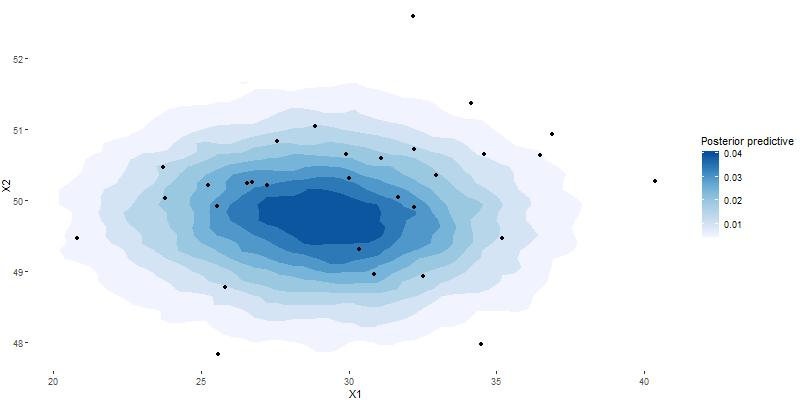
\includegraphics[scale=0.4]{density-predictive-full-X.jpeg}
  \end{center}
  \end{figure}

\section{Introduction}

\urllink{Overleaf}{https://www.overleaf.com/} is popular online \LaTeX{}
editor. It can generate PDF files 
without need to install a local \TeX{} distribution. Unfortunatelly, it doesn't
support conversion to HTML out of the box. To get the HTML version of the
document, we must use some tricks.

There are many tools that support the conversion from \LaTeX{} to HTML, each of
them use a different approach. I am a developer of
\urllink{\TeX4ht}{https://tug.org/tex4ht/}, so I will present solution that
uses this tool. 

\TeX4ht uses \TeX{} for the actual conversion. It loads special configuration
files for internal \LaTeX{} code or for the used packages. These configuration
files patch commands with special instructions that insert HTML (or other
supported formats). Because it uses \TeX{} for the actual conversion, it
supports custom commands. It also supports font changing commands, so  it
doesn't need custom configurations in many cases.

The first method that use \TeX4ht for the conversion was presented by LianTze
Lim. It uses a custom build file for
\urllink{Latexmk}{https://www.overleaf.com/latex/examples/testing-html-export-with-tex4ht/rqcknjvwyyry} 
that calls \TeX4ht. The downside is that the generated HTML file is not easilly accessible.  

To make the conversion easier, I've set up \urllink{Docker image}{https://hub.docker.com/repository/docker/michalh21/make4ht-docker/general} for \TeX4ht. 
Thanks to \urllink{GitHub Actions}{https://help.github.com/en/actions/automating-your-workflow-with-github-actions/about-github-actions}, 
it is possible to use this image for the conversion of the Overleaf document to HTML. 
The generated files can be published on the web using Github Pages, where they can be automatically 
updated on every document change. This document is an example of this setup.

\section{Setup}

\subsection{On Overleaf}

First step is to sync your Overleaf project with your GitHub account, following \foothref{a guide on 
  Overleaf}{https://www.overleaf.com/learn/how-to/How_do_I_connect_an_Overleaf_project_with_a_repo_on_GitHub,_GitLab_or_BitBucket\%3F}
{\texttt{https://www.overleaf.com/learn/how-to/How\_do\_I\_connect\_an\_Overleaf\_project\_with\_a\allowbreak\_repo\_on\_GitHub,\_GitLab\_or\_BitBucket\%3F}}. 
Don't forget to run the \cmdname{Sync -> GitHub} command from Overleaf main menu every time you had updated the document.

\subsection{On GitHub}
Next step is to configure actions in the Github project created for your
document. Two steps are necessary -- first  one compiles the document to HTML
using \TeX4ht, the second step publishes the generated HTML files on the Web
using \urllink{GitHub Pages}{https://pages.github.com/}

For the web publishing we  use the \verb|actions-gh-pages|
\urllink{action}{https://github.com/peaceiris/actions-gh-pages}. 

When the keys are set up, you can create the workflow file. Select the
\cmdname{Actions} tab and click the \cmdname{Set up a workflow yourself}
button. It will open an editor with a YAML file for the Action workflow.
Replace it with the following content:

% I am just testing if this command works in the container
\AtEndEnvironment{lstlisting}{\relax}

\begin{lstlisting}{yaml}
name: CI
on: [push]
jobs:
  build:
    runs-on: ubuntu-latest
    steps:
    - uses: actions/checkout@v1
    - name: Run make4ht
      uses: docker://ghcr.io/michal-h21/make4ht-action:latest
      env:
        command: "make4ht -u -d out main.tex"
    - name: Publish the web pages
      uses:  peaceiris/actions-gh-pages@v3
      with:
        github_token: ${{ secrets.GITHUB_TOKEN }}
        publish_dir: ./out
\end{lstlisting}

The important part of the configuration is the \cmdname{command} key. It
contains the actual command used for the compilation. We use
\urllink{Make4ht}{https://ctan.org/pkg/make4ht?lang=en}, build system for
\TeX4ht.

Command \verb|"make4ht -u -d out main.tex"| creates UTF-8 encoded HTML file
from the \cmdname{main.tex} input file. The \texttt{-d} option specifies the
output directory for the HTML files. This directory will be used for the web
publishing and should be passed to the \verb|publish_dir| key in
\textit{Publish the web pages} step.

The web will be published at \url{https://yourgitubusename.github.io/project_name/main.html}. 
\section{Links}
\begin{itemize}
    \item This document: \url{https://www.kodymirus.cz/overleaf-html-sample/main.html}
    \item Source repository: \url{https://github.com/michal-h21/overleaf-html-sample} 
\end{itemize}
 



\end{document}
